% To do:
% Wei: Recurrent layer is concatnateded or added with the previous layers?. (add)
% Do we need to mention the norm?

\section{Model Architecture}

\begin{figure}[htb]
\begin{center}
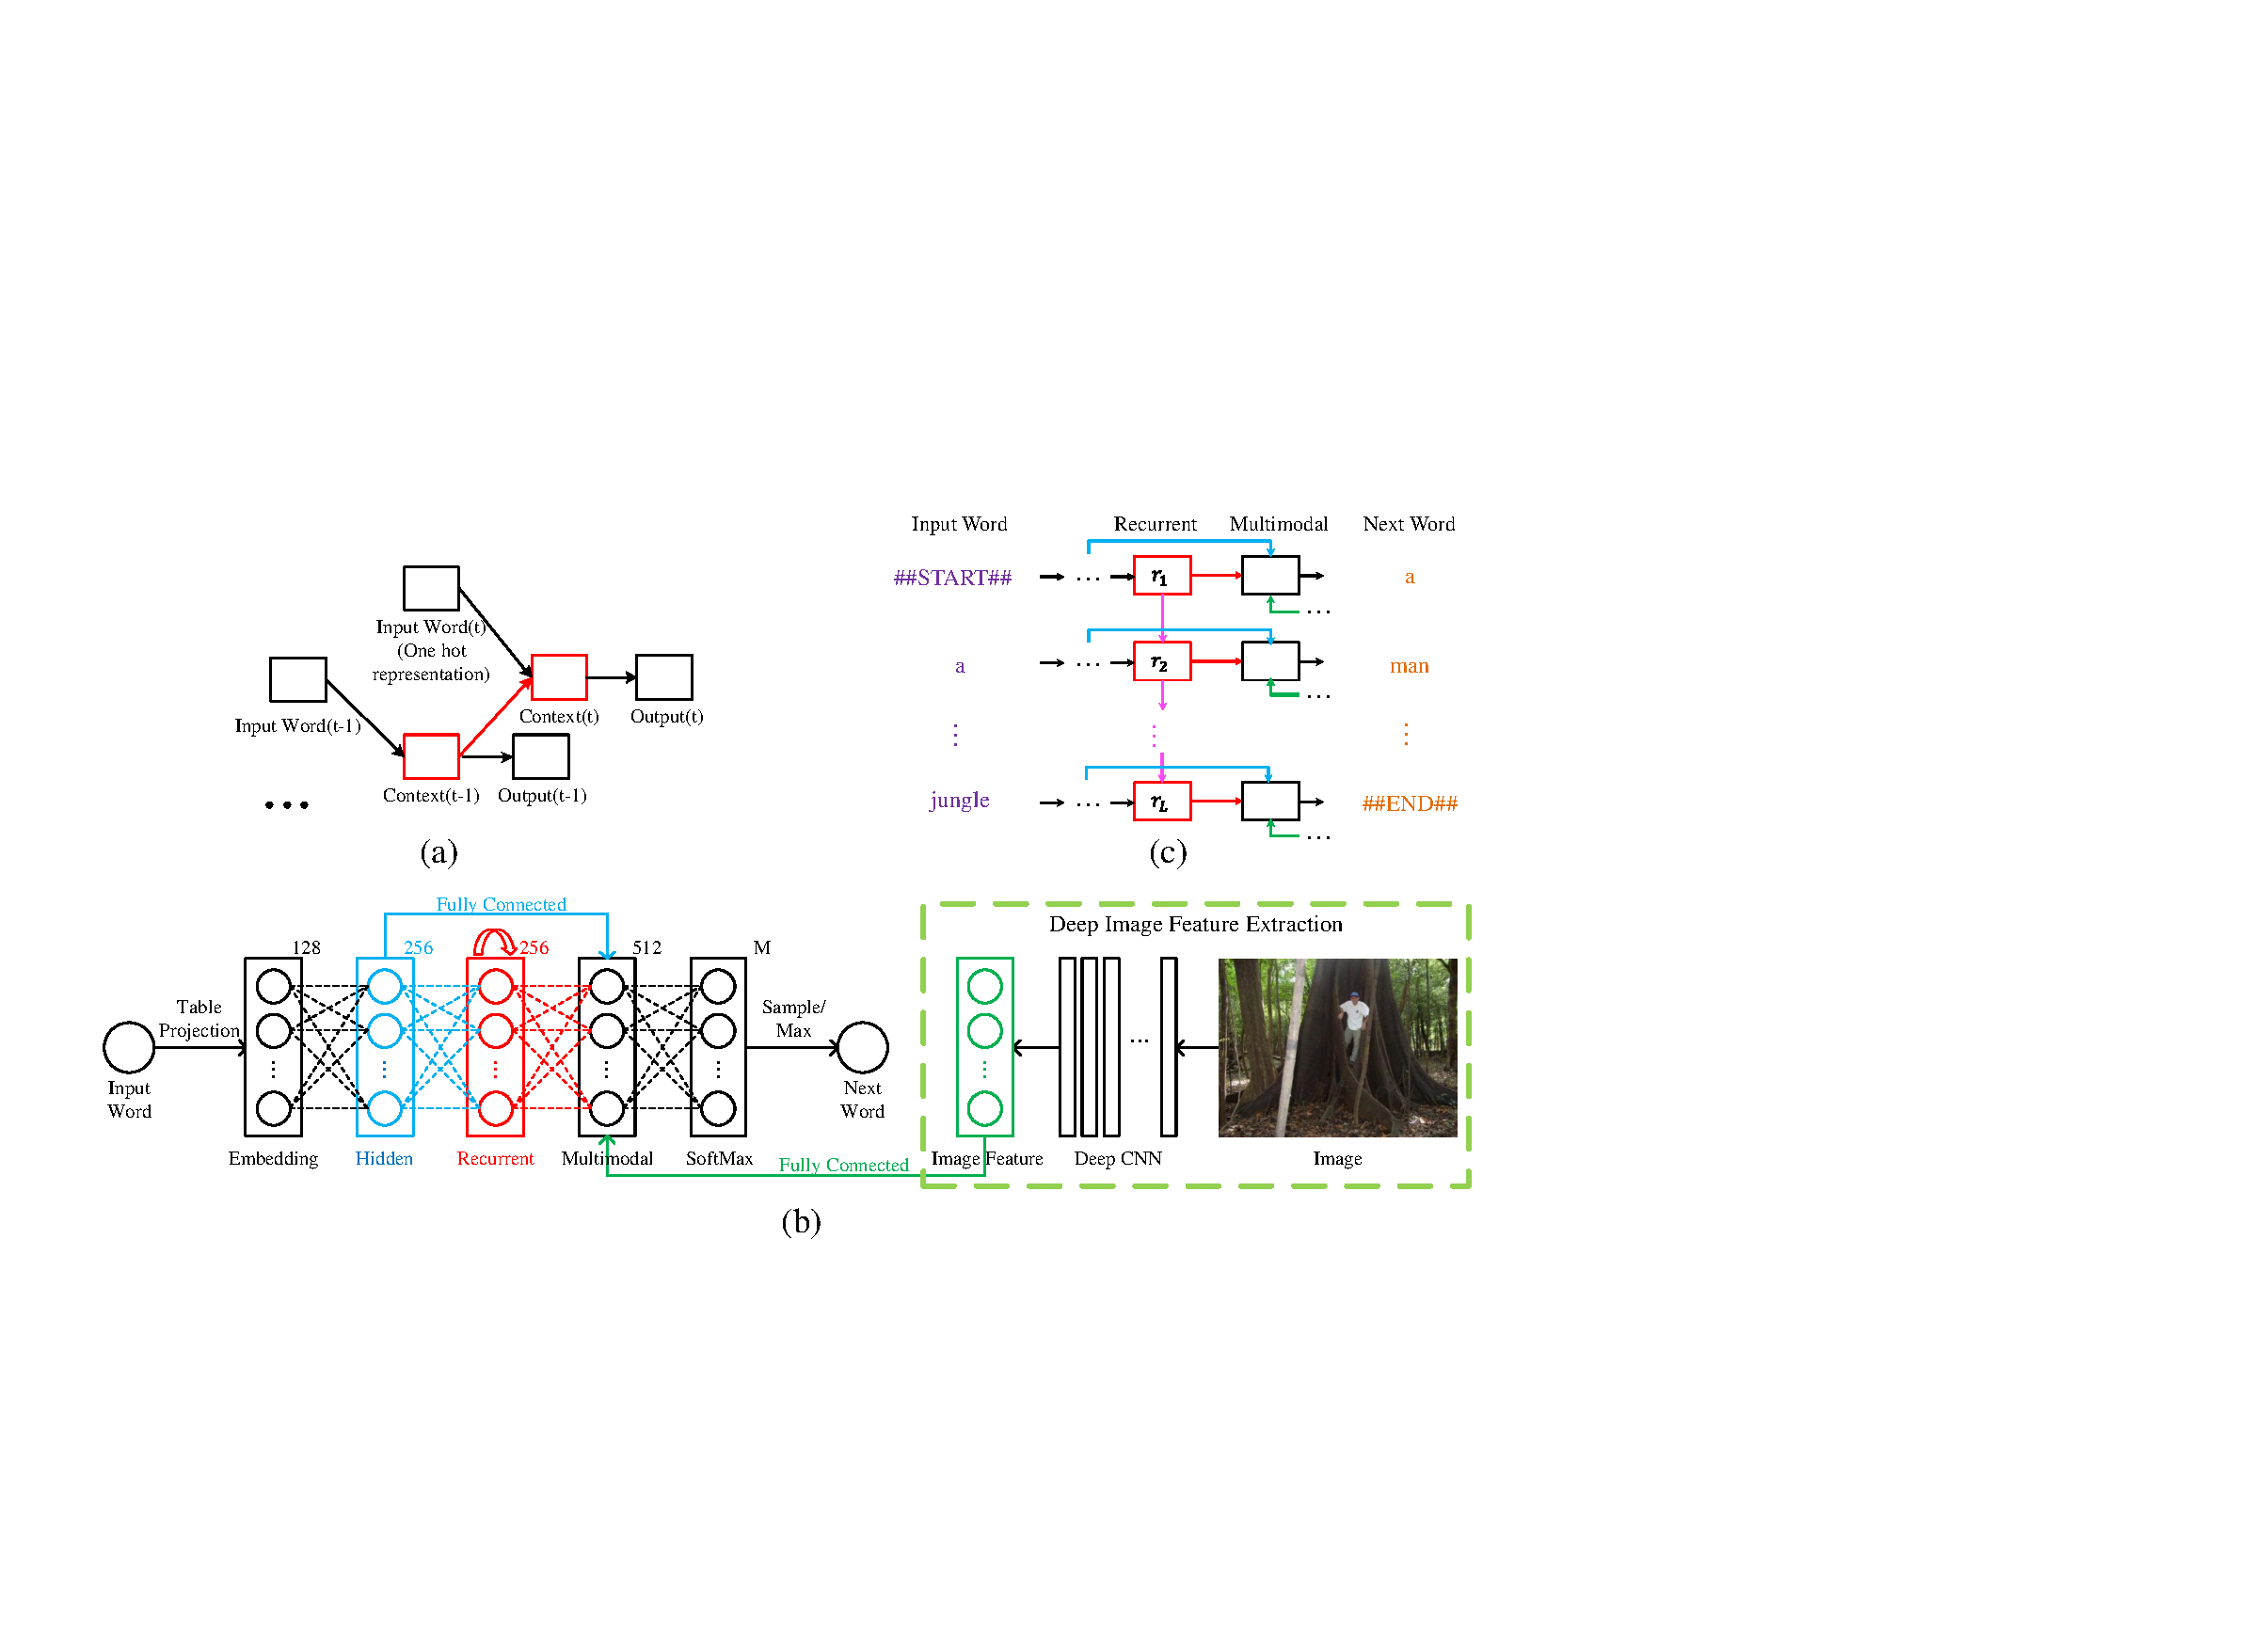
\includegraphics[width=0.95\linewidth]{PaperFigures/arch_final_visio.pdf}
\end{center}
   \caption{Illustration of the simple Recurrent Neural Network (RNN) and our multimodal Recurrent Neural Network (m-RNN) architecture.
   (a). The simple RNN. 
   (b). Our m-RNN model.
   The input of our model is an image and its corresponding sentences (e.g. the sentence for the shown image is: \emph{a man at a giant tree in the jungle}).
   The model will estimate the probability distribution of the next word given previous words and the image.
   This architecture is much deeper than the simple RNN.
   % of structure without considering the extendibility of the recurrent layer.
   (c). The illustration the unfolded m-RNN. 
   % We can unfold the recurrent layer, which leads to the temporal depth of the network.
   The model parameters are shared for each temporal frame of the m-RNN model.
   }
\label{fig:illu_RNN}
\end{figure}

% For layer \textcircled{\raisebox{-0.9pt}{1}} and layer \textcircled{2},
\subsection{Simple recurrent neural network}
\label{sec:sRNN}
We briefly introduce the simple Recurrent Neural Network (RNN) or Elman network \cite{elman1990finding} that is widely used for many natural language processing tasks, such as speech recognition \cite{mikolov2010recurrent,mikolov2011extensions}.
Its architecture is shown in Figure \ref{fig:illu_RNN}(a).
It has three types of layers in each time frame: the input word layer $\mathbf{w}$, the recurrent layer $\mathbf{r}$ and the output layer $\mathbf{y}$.
The activation of input, recurrent and output layers at time $t$ is denoted as $\mathbf{w}(t)$, $\mathbf{r}(t)$, and $\mathbf{y}(t)$ respectively.
$\mathbf{w}(t)$ is the one-hot representation of the current word. 
This representation is binary, and has the same dimension of the vocabulary size with only one non-zero element.
$y(t)$ can be calculated as follows:
\begin{equation}
\mathbf{x}(t) = [\mathbf{w}(t)\ \ \mathbf{r}(t-1)];\ \ \ 
\mathbf{r}(t)=f_1(\mathbf{U} \cdot \mathbf{x}(t));\ \ \ 
\mathbf{y}(t)=g_1(\mathbf{V} \cdot \mathbf{r}(t));
\end{equation}
where $\mathbf{x}(t)$ as a vector that concatenates $\mathbf{w}(t)$ and $\mathbf{r}(t-1)$, $f_1(.)$ and $g_1(.)$ are element-wised sigmoid and softmax function respectively, and $\mathbf{U}$, $\mathbf{V}$ are weights which will be learned.

The size of RNN is adaptive to the length of the input sequence and the recurrent layers connect the sub-networks in different time frames.
Accordingly, when we do the backpropagation, we need to propagate the error through recurrent connections back in time \cite{rumelhart1988learning}.

%We define two types of ``depths'' for a RNN architecture. 
%We denote the number of layers in each time session as the \emph{structure depth} (e.g. the structure depth of the basic RNN is 3).
%When we compare the depth of different RNN networks, we refer to the structure depth.
%The second depth is denoted as the \emph{temporal depth}. 
% Although the structure of the basic RNN model is simple, it is a very deep network which can be unfolded in time sequences.

\subsection{Our m-RNN model}
The structure of our multimodal Recurrent Neural Network (m-RNN) is shown in Figure \ref{fig:illu_RNN}(b).
The m-RNN model is much deeper than the simple RNN model.
It has six layers in each time frame: the input word layer, two word embedding layers, the recurrent layer, the multimodal layer, and the softmax layer).

The two word embedding layers embed the one-hot input into a dense word representation.
It has several advantages.
Firstly, it will significantly lower the number of parameters in the networks because the dense word vector (128 dimension) is much smaller than the one-hot word vector.
Secondly, the dense word embedding encodes the semantic meanings of the words \cite{mikolov2013efficient}.
The semantically relevant words can be found by calculating the Euclidean distance between two dense word vectors in embedding layers.

Most of the sentence-image multimodal models \cite{karpathy2014fragment,frome2013devise,socher2014grounded,kiros2013multimodal} use pre-computed word embedding vectors as the initialization of their model. 
In contrast, we randomly initialize our word embedding layers and learn them from the training data.
We show that this random initialization is sufficient for our architecture to generate the state-of-the-art results.
% To further refine the word representation, we add a hidden layer after the initial word embedding layer and 
We treat the activation of the word embedding layer 2 (see Figure \ref{fig:illu_RNN}(b)) as the final word representation, which directly inputs in the multimodal layer.

After the two word embedding layers, we have a recurrent layer with 256 dimensions.
The calculation of the recurrent layer is slightly different from the calculation for the simple RNN.
Instead of concatenating the word representation at time $t$ (denoted as $\mathbf{w}(t)$) and the recurrent layer activation at time $t-1$ (denoted as $\mathbf{r}(t-1)$), we first map $\mathbf{r}(t-1)$ into the same vector space as $\mathbf{w}(t)$ and add them together:
\begin{equation}
\mathbf{r}(t)=f_2(\mathbf{U}_r \cdot \mathbf{r}(t-1) + \mathbf{w}(t));
\end{equation}
% where $\mathbf{s}$ and $\mathbf{w}$ denotes the recurrent layer vector and the word representation respectively.
% This strategy will reduce the number of parameters and accelerate the training and testing process.
We set $f_2(.)$ as the Rectified Linear Unit (ReLU), inspired by its the recent success when training very deep structure in computer vision field \cite{krizhevsky2012imagenet}.
This differs from the simple RNN where the sigmoid function is adopted (see Section \ref{sec:sRNN}).
ReLU is faster, and harder to saturate or overfit the data than non-linear functions like the sigmoid.
When backpropagation through time (BPTT) \cite{rumelhart1988learning} is conducted for RNN with sigmoid function, the vanishing gradient problem appears since even the simplest RNN model can have a large temporal depth.
Previous methods \cite{mikolov2010recurrent,mikolov2011extensions} used heuristics, such as truncated BPTT, to avoid this problem.
Truncated BPTT stops the BPTT after $k$ time steps, where $k$ is a hand-defined hyperparameter.
Because of the good properties of ReLU, we do not need to stop the BPTT at an early stage, which leads to a better and more efficient utilization of the data than truncated BPTT.

After the recurrent layer, we set up a 512 dimensional multimodal layer that connect the language model part and the image part of the m-RNN model (see Figure \ref{fig:illu_RNN}(b)).
The language model part includes the word embedding layer 2 (the final word representation) and the recurrent layer (the sentence context).
The image part contains the image feature extraction network.
Here we connect the seventh layer of AlexNet \cite{krizhevsky2012imagenet} to the multimodal layer (please refer to Section \ref{sec:ImgSenFeat} for more details).
But our framework can use any image features.
We map the feature vector for each layer to the same feature space and add them together to obtain the feature vector for the multimodal layer:
\begin{equation}
\mathbf{m}(t)=g_2(\mathbf{V}_w \cdot \mathbf{w}(t) + \mathbf{V}_r \cdot \mathbf{r}(t) + \mathbf{V}_I \cdot \mathbf{I});
\end{equation}
where $\mathbf{m}$ denotes the multimodal layer feature vector, $\mathbf{I}$ denotes the image feature, $g_2(.)$ is the element-wised scaled hyperbolic tangent function \cite{lecun2012efficient}:
\begin{equation}
g_2(x) = 1.7159 \cdot \tanh( \frac{2}{3} x)
\end{equation}
This function forces the gradients into the most non-linear value range and accelerates the training process than the basic hyperbolic tangent function.

%We do not restrict the norm the three feature layers that connect to the multimodal layer.
%Our experiments shows that the L2 norm of the hidden layer, 

As the simple RNN, our m-RNN model has a softmax layer that will generate the probability distribution of the next word.
The dimension of this layer is the vocabulary size $M$, which is different for different datasets.

\section{Training the m-RNN}
\label{sec:trainCost}
For training our m-RNN model we adopt a cost function based on the \emph{Perplexity} of the sentences in the training set given their corresponding images.
Perplexity is a standard measure for evaluating language model.
The perplexity for one word sequence (i.e. a sentences) $w_{1:L}$ is calculated as follows:
\begin{equation}
\log_2 \mathcal{PPL}(w_{1:L}|\mathbf{I}) = -\frac{1}{L} \sum_{n=1}^{L} \log_2 P(w_n|w_{1:n-1},\mathbf{I})
\end{equation}
where $L$ is the length of the word sequences, $\mathcal{PPL}(w_{1:L}|\mathbf{I})$ denotes the perplexity of the sentence $w_{1:L}$ given the image $\mathbf{I}$.
$P(w_n|w_{1:n-1},\mathbf{I})$ is the probability of generating the word $w_n$ given $\mathbf{I}$ and previous words $w_{1:n-1}$.
It corresponds to the feature vector of the SoftMax layer of our model.

The cost function of our model is the average log-likelihood of the words given their context words and corresponding images in the training sentences plus a regularization term.
It can be calculated by the perplexity:
\begin{equation}
\mathcal{C} = \frac{1}{N} \sum_{i=1}^{N} L \cdot \log_2 \mathcal{PPL}(w_{1:L}^{(i)}|\mathbf{I}^{(i)}) + \left \| \theta \right \|_2^2
\end{equation}
where $N$ is the number of words in the training set and $\theta$ is the model parameters.
% It is equivalent to the reciprocal of the geometric mean of the probability to generate the training sentences using the model.

Our training objective is to minimize this cost function, which is equivalent to maximize the probability of the model to generate the sentences in the training set given their corresponding images.
The cost function is differentiable and we use backpropagation to learn the model parameters.

\section{Learning of Sentence and Image Features}
\label{sec:ImgSenFeat}

The architecture of our model allows the gradients from the loss function to be backpropagated to both the language modeling part (i.e. the word embedding layers and the recurrent layer) as well as the image part (e.g. the AlexNet \cite{krizhevsky2012imagenet}).

For the language modeling part, as mentioned above, we randomly initialize the language modeling layers and learn their parameters. For the image part, we connect the seventh layer of a pre-trained Convolutional Neural Network \cite{krizhevsky2012imagenet,donahue2013decaf} (denoted as AlexNet).
The same features extracted from the seventh layer of AlexNet (also denoted as decaf features \cite{donahue2013decaf}) are widely used by previous multimodal methods \cite{kiros2013multimodal,frome2013devise,karpathy2014fragment,socher2014grounded}.
A recent multimodal retrieval work \cite{karpathy2014fragment} showed that using the RCNN object detection framework \cite{girshick2014rcnn} combined with the decaf features significantly improves the performance.
In the experiments, we show that our method performs much better than \cite{karpathy2014fragment} when the same image features are used, and is better than or comparable to their results even when they use more sophisticated features based on object detection.

We can update the AlexNet according to the gradient backpropagated from the multimodal layer. In this paper, we fix the image features and the deep CNN network in the training stage due to a shortage of data (The datasets we used in the experiment have less than 30K images).
In future work, we will apply our method on large datasets and finetune the parameters of the deep CNN network in the training stage.

\section{Sentence Generation, Image and Sentence Retrieval}
We can use the trained m-RNN model for three tasks: 1) Sentences generation; 2) Sentence retrieval (retrieving most relevant sentences to the given image); 3) Image retrieval (retrieving most relevant images to the given sentence);

The sentence generation process is straightforward.
Start from the start sign ``\#\#START\#\#'' or arbitrary number of reference words (e.g. we can input the first K words in the reference sentence to the model and then start to generate new words), our model can calculate the probability distribution of the next word: $P(w|w_{1:n-1},\mathbf{I})$.
Then we can sample from this probability distribution to pick the next word.
In practice, we find that selecting the word with the maximum probability performs slightly better than sampling.
After that, we input the picked word to the model and continue the process until the model outputs the end sign ``\#\#END\#\#''.

For the retrieval tasks, we use our model to calculate the perplexity of generating a sentence given an image.
The perplexity can be treated as an affinity measurement between sentences and images.
For the image retrieval task, we rank the images based on their perplexity with the query sentence and output the top ranked ones. 

The sentence retrieval task is trickier because there might be some sentences that have high probability for any image query (e.g. sentences consists of many frequently appeared words).
Instead of looking at the perplexity or the probability of generating the sentences given the query image, we use the normalized probability for each sentence: $P(w_{1:L}|\mathbf{I}) / P(w_{1:L})$.
$P(w_{1:L}) = \sum_{\mathbf{I^{'}}} P(w_{1:L}|\mathbf{I^{'}}) \cdot P(\mathbf{I^{'}})$, where $\mathbf{I^{'}}$ are images sampled from the training set.
We approximate $P(\mathbf{I^{'}})$ by a constant and ignore this term.
$P(w_{1:L}|\mathbf{I}) = \mathcal{PPL}(w_{1:L}|\mathbf{I}) ^ {-L}$.